\documentclass[11pt,letterpaper]{article}
\usepackage[margin=1in]{geometry}
\usepackage{graphicx,booktabs,tabularx,array,xcolor,amsmath,enumitem,titlesec,fancyhdr}
\usepackage[hidelinks]{hyperref}
\usepackage[most]{tcolorbox}
\usepackage{float}

\definecolor{accent}{HTML}{1F3A5F}
\titleformat{\section}{\large\bfseries\color{accent}}{\thesection.}{0.5em}{}
\titleformat{\subsection}{\normalsize\bfseries}{}{0em}{}
\setlist{itemsep=2pt,topsep=4pt}
\setlength{\parskip}{5pt}\setlength{\parindent}{0pt}
\pagestyle{fancy}\fancyhf{}\renewcommand{\headrulewidth}{0pt}
\fancyfoot[L]{\small\color{gray}Canadian Bank Credit Stress Test}\fancyfoot[R]{\small\color{gray}\thepage}
\newcolumntype{Y}{>{\raggedright\arraybackslash}X}

\begin{document}

{\color{accent}\LARGE\bfseries Canadian Bank Credit Stress Test}\\[4pt]
{\large Projecting credit losses and capital for Canada's Big 6 banks under recession and stagflation}\\[8pt]
{\small Esther Wong \quad$\cdot$\quad October 2026 \quad$\cdot$\quad Jump-off: fiscal Q3 2026 (calendar 2026Q2)}

\vspace{6pt}
\begin{tcolorbox}[colback=accent!5,colframe=accent,boxrule=0.6pt,arc=2pt,title=\textbf{Key results},fonttitle=\small]
\small
\begin{itemize}[leftmargin=12pt]
  \item \textbf{Scope:} 9-quarter credit losses and CET1 capital for RBC, TD, Scotiabank, BMO, CIBC and National Bank under base, adverse-recession and severe-stagflation scenarios.
  \item \textbf{Losses:} under severe stagflation (unemployment +4pp to 10.7\%, house prices $-$30\%, policy rate +200bp), the Big 6 lose \textbf{C\$43.5bn} on Canadian loans over 9 quarters.
  \item \textbf{Most exposed: Scotiabank.} CET1 falls 162bp to 11.47\%, just under OSFI's 11.5\% expectation, driven by its international book and a thinner earnings cushion.
  \item \textbf{Least exposed: RBC.} Earnings absorb its losses and CET1 ends where it started.
  \item \textbf{Robust ranking:} a macro regression and a Vasicek default model, built independently, identify the same two most and two least exposed banks.
\end{itemize}
\end{tcolorbox}

\section{Objective}
Regulators stress-test banks to check they can absorb losses in a severe downturn and still meet capital requirements. This project builds a simplified version of that exercise for Canada's six largest banks: project credit losses on their Canadian loan books under three economic scenarios, net them against earnings, and track each bank's Common Equity Tier 1 (CET1) ratio against OSFI's 11.5\% expectation for domestic systemically important banks.

\section{Data}
\begin{center}\small
\begin{tabularx}{\linewidth}{@{}l Y Y@{}}
\toprule
Data & Source & Notes \\
\midrule
Provisions (PCL), loans, capital & Banks' Supplementary Financial Information packages & $\sim$70 quarterly packages, fiscal 2018 onward (the IFRS 9 era); parsed from Excel, and from PDF for older TD, Scotiabank and BMO quarters \\
Unemployment, real GDP & Statistics Canada (tables 14-10-0287, 36-10-0104) & Quarterly \\
Policy rate & Bank of Canada Valet API & Overnight rate target \\
House prices & BIS residential property prices & Canada, nominal \\
\bottomrule
\end{tabularx}
\end{center}

Each bank's quarterly PCL and loans are mapped to three Canadian portfolios: \textbf{mortgages and HELOCs}, \textbf{consumer} (cards, personal lending) and \textbf{business}. The result is a panel of 6 banks $\times$ 3 portfolios $\times$ 35 quarters (2017Q4--2026Q2). Banks disclose differently, so some splits had to be allocated; for example, Scotiabank publishes no loans or PCL by geography, so its ``Canada'' is the Canadian Banking segment. Every allocation is logged in the project's decisions file, and automated checks flag large quarter-on-quarter moves in loans (relabels or acquisitions) and large provision releases.

\begin{figure}[H]\centering
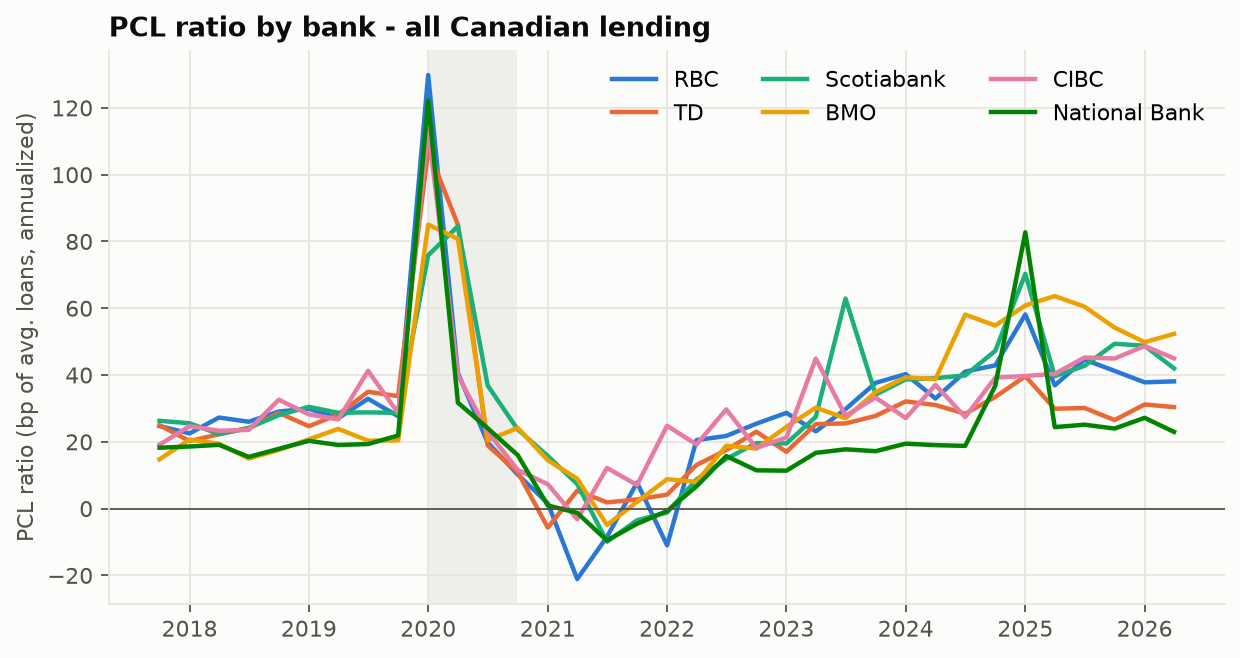
\includegraphics[width=0.85\linewidth]{figures/pcl_history.png}
\caption{Historical PCL ratio by bank, all Canadian lending; the shaded band marks the COVID provisioning spike.}
\end{figure}

\section{Scenarios}
Three 9-quarter paths start from 2026Q2. The adverse scenario is a conventional recession with rate cuts; stagflation combines a deeper recession with \emph{rising} rates, which removes the usual relief to borrowers.

\begin{table}[H]\centering\small
\caption{Scenario paths (peak or trough versus jump-off)}
\begin{tabular}{@{}lrrrr@{}}\toprule
Scenario & Unemployment peak & GDP & House prices & Policy rate (end) \\ \midrule
Base & 6.65\% & +0.5\% & +0.1\% & 2.25\% \\
Adverse recession & 9.67\% (+3.0pp) & $-$3.0\% & $-$20\% & 0.50\% \\
Severe stagflation & 10.67\% (+4.0pp) & $-$4.0\% & $-$30\% & 4.25\% \\ \bottomrule
\end{tabular}
\end{table}

\section{Method}
Losses are projected with two independent models. The headline uses the \textbf{average} of the two; each can also be run on its own.

\subsection{Method A: macro satellite regression}
For each portfolio, a panel regression across the six banks links the quarterly PCL ratio to the economy:
\[
\text{PCL}_{b,t} = \alpha_b + \beta' X_t + \rho\,\text{PCL}_{b,t-1} + \varepsilon_{b,t}
\]
where $\alpha_b$ is a bank fixed effect and $X_t$ holds three macro variables chosen per portfolio (change in unemployment, house price or GDP growth, and the lagged policy rate). Standard errors are clustered by quarter, because the macro variables are shared by all banks. Every coefficient has the sign economic theory requires.

\begin{table}[H]\centering\small
\caption{Satellite regression results (PCL in bp of loans; $n = 204$ per portfolio)}
\begin{tabular}{@{}lrrr@{}}\toprule
 & Mortgages & Consumer & Business \\ \midrule
$\Delta$ unemployment (pp) & 0.25$^{**}$ & 9.83 & 4.11$^{*}$ \\
House price growth, lag 1 (\%) & $-$0.04$^{**}$ & -- & -- \\
GDP growth (\%) & -- & $-$1.34 & $-$3.11$^{**}$ \\
Policy rate, lag 2 (\%) & 0.20 & 16.44$^{***}$ & 5.76$^{***}$ \\
Lagged PCL ratio & 0.33$^{***}$ & 0.30$^{**}$ & 0.02 \\ \midrule
$R^2$ & 0.42 & 0.48 & 0.33 \\ \bottomrule
\multicolumn{4}{@{}l}{\footnotesize $^{*}p<0.1$, $^{**}p<0.05$, $^{***}p<0.01$.}
\end{tabular}
\end{table}

The regression's weakness is its history: the IFRS 9 sample contains one real downturn (COVID), cushioned by government support, so coefficients are unstable across sub-periods and the model tends to understate severe losses.

\subsection{Method B: Vasicek single-factor model}
The Vasicek model, the basis of Basel capital rules, converts a through-the-cycle default probability into a stressed one given a systematic economic shock $z$:
\[
\text{PD}_{\text{stressed}} = \Phi\!\left( \frac{\Phi^{-1}(\text{PD}_{\text{base}}) - \sqrt{\rho}\, z}{\sqrt{1-\rho}} \right)
\]
The scenario's unemployment path drives $z$. Asset correlations follow Basel ($\rho$ = 0.15 mortgages, 0.04 consumer, 0.18 business). Losses are stressed PD $\times$ loss given default (LGD); mortgage LGD rises as house prices fall, consumer and business LGDs are fixed (75\% and 40\%). The unemployment-to-$z$ mapping was calibrated so that 2008--10 conditions reproduce roughly 2009 loss levels.

\subsection{From losses to capital}
Each quarter, pre-tax income = pre-provision earnings (cut 20\% in the adverse and 25\% in the stagflation scenario) $-$ Canadian credit losses $-$ non-Canadian provisions (stressed in proportion to each bank's Canadian loss multiple). After tax at 26.5\% and dividends held at their trailing level, the result is added to CET1 capital, while risk-weighted assets grow with credit migration. The CET1 ratio path is then compared with OSFI's 11.5\% expectation (8\% regulatory floor plus the 3.5\% Domestic Stability Buffer).

\section{Results}

\begin{table}[H]\centering\small
\caption{Canadian credit losses, 9-quarter cumulative (bp of loans)}
\begin{tabular}{@{}lrrrr@{}}\toprule
Scenario & Mortgages + HELOCs & Consumer & Business & Total (C\$bn) \\ \midrule
Base & 6 & 330 & 71 & 21.3 \\
Adverse recession & 12 & 399 & 153 & 32.7 \\
Severe stagflation & 23 & 490 & 208 & 43.5 \\ \bottomrule
\end{tabular}
\end{table}

\begin{figure}[H]\centering
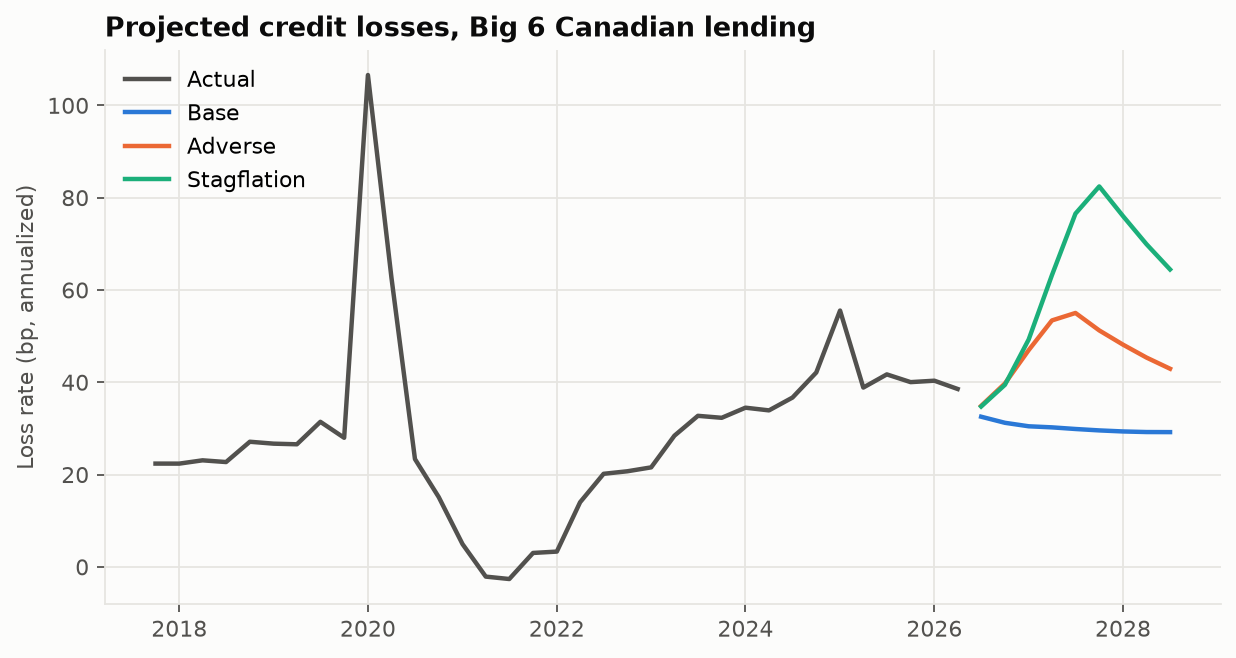
\includegraphics[width=0.85\linewidth]{figures/loss_paths.png}
\caption{Big 6 Canadian lending: actual loss rate since 2018 and projected loss rate under each scenario.}
\end{figure}

Consumer lending drives most losses; mortgages stay low even with house prices down 30\%, because insured mortgages and large equity cushions limit losses. Before earnings, Canadian credit losses alone would consume 96--150bp of CET1 under stagflation (after tax). National Bank and CIBC are hit hardest at this stage because they are the most concentrated in Canada; earnings power is what separates them afterwards.

\begin{table}[H]\centering\small
\caption{CET1 under severe stagflation (headline: average of both methods)}
\begin{tabular}{@{}clrrrrl@{}}\toprule
Rank & Bank & Start & Low & Drawdown & vs 11.5\% & Main driver \\ \midrule
1 & Scotiabank & 13.1\% & 11.47\% & 162bp & $-$3bp & Non-Canadian book \\
2 & TD & 14.3\% & 13.1\% & 116bp & +161bp & Non-Canadian book \\
3 & BMO & 13.0\% & 12.0\% & 104bp & +46bp & Non-Canadian book \\
4 & National Bank & 13.5\% & 12.6\% & 95bp & +106bp & Business \\
5 & CIBC & 13.4\% & 13.3\% & 7bp & +183bp & Consumer \\
6 & RBC & 13.5\% & 13.5\% & $-$4bp & +203bp & Business \\ \bottomrule
\end{tabular}
\end{table}

Under the adverse recession every bank stays well above 11.5\%; Scotiabank's drawdown is 77bp and RBC's and CIBC's ratios rise slightly.

\begin{figure}[H]\centering
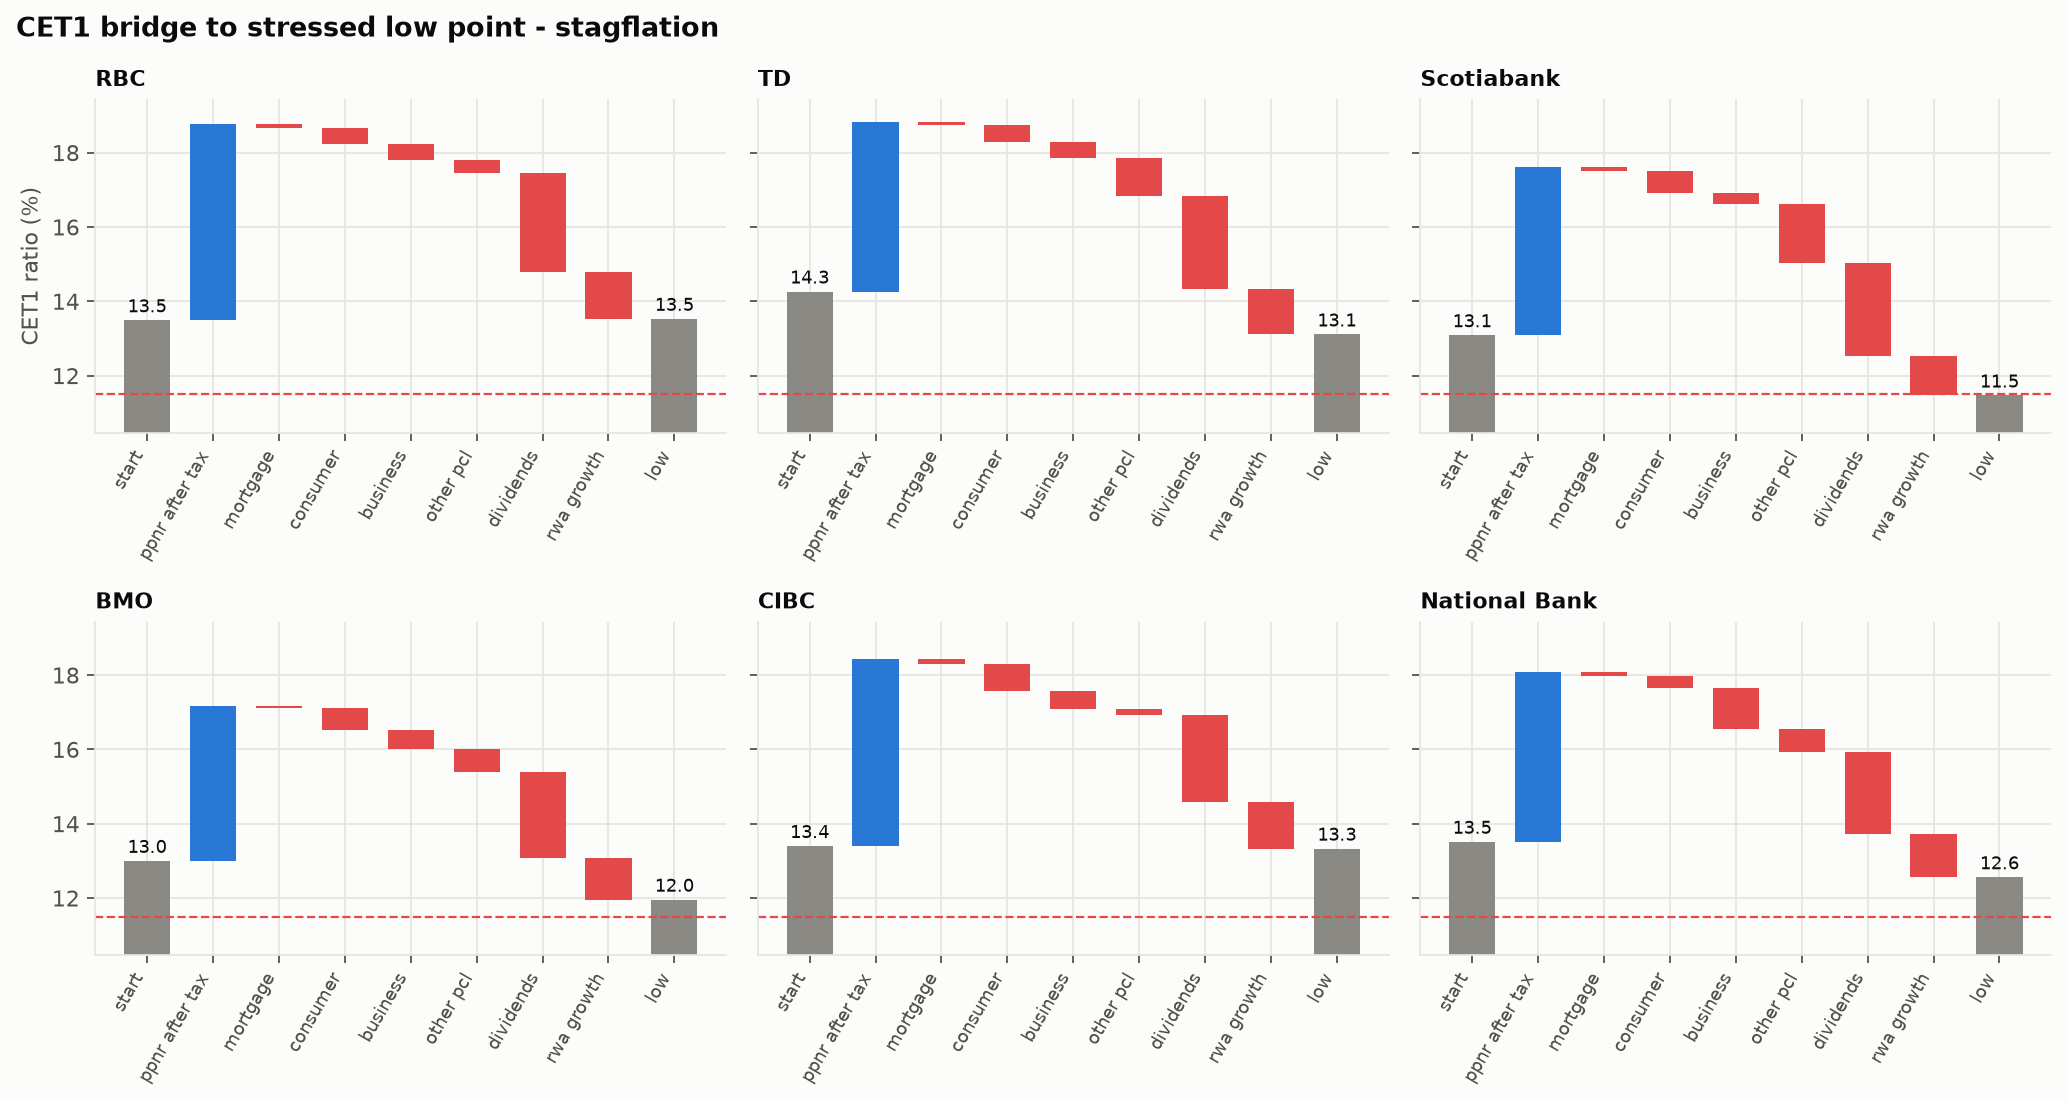
\includegraphics[width=0.85\linewidth]{figures/cet1_waterfall_stagflation.png}
\caption{CET1 bridge to the stressed low point under severe stagflation: starting ratio, after-tax pre-provision earnings, Canadian losses by portfolio, other provisions, dividends and RWA growth.}
\end{figure}

\begin{figure}[H]\centering
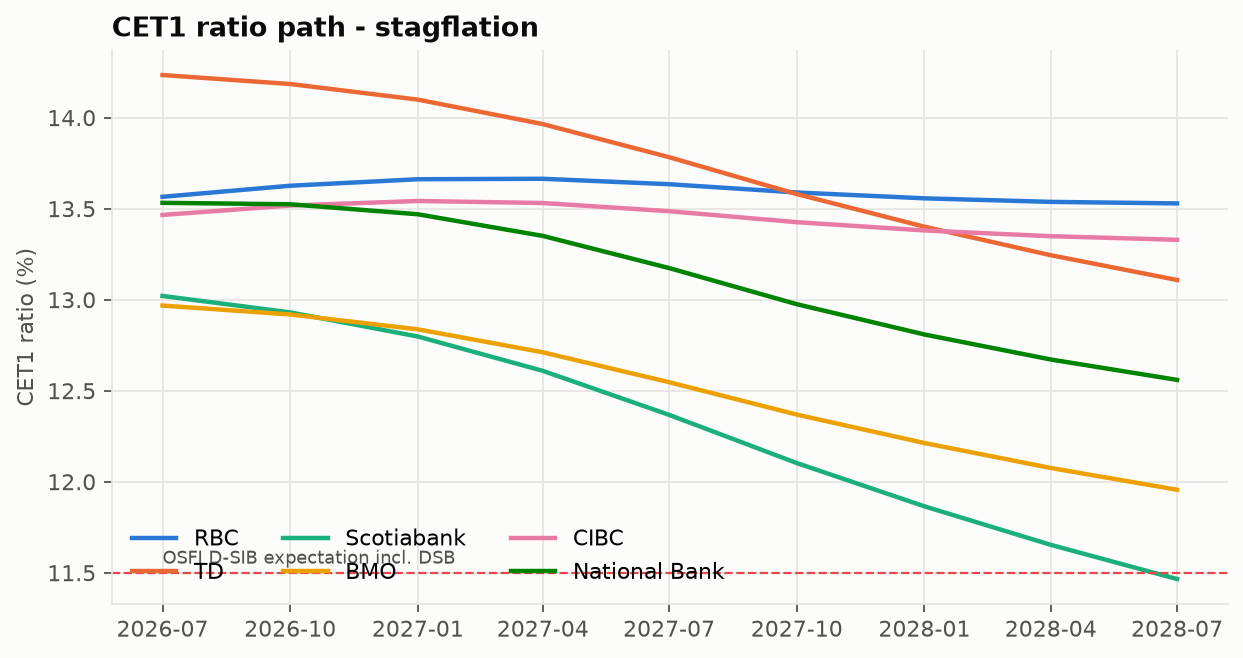
\includegraphics[width=0.85\linewidth]{figures/cet1_paths_stagflation.png}
\caption{CET1 ratio paths under severe stagflation against OSFI's 11.5\% expectation.}
\end{figure}

\section{Robustness}
\textbf{Ranking across methods.} The two methods differ in level but agree on who is most and least exposed:

\begin{table}[H]\centering\small
\caption{Stagflation ranking by method (1 = most exposed)}
\begin{tabular}{@{}clll@{}}\toprule
Rank & Regression & Vasicek & Average \\ \midrule
1 & Scotiabank & Scotiabank & Scotiabank \\
2 & TD & TD & TD \\
3 & BMO & National Bank & BMO \\
4 & National Bank & BMO & National Bank \\
5 & CIBC & CIBC & CIBC \\
6 & RBC & RBC & RBC \\ \bottomrule
\end{tabular}
\end{table}

\textbf{Method agreement.} In the base case the two models give similar losses (Vasicek 0.7--2.2$\times$ the regression, depending on bank and portfolio). Under stress they diverge: Vasicek losses are 1.1--2.6$\times$ the regression for consumer loans, 2.6--4.8$\times$ for business loans and 2.1--7.1$\times$ for mortgages. The gap reflects the regression's thin downturn history rather than a flaw in either model, and averaging the two is a deliberate middle ground.

\section{Limitations}
\begin{itemize}[leftmargin=12pt]
  \item \textbf{One downturn in the data.} The IFRS 9 sample has only COVID, cushioned by government support; regression coefficients are unstable across sub-periods.
  \item \textbf{Allocated data.} Several banks do not disclose provisions by Canadian product, so parts of the panel are allocated; Scotiabank's Canadian scope is its Canadian Banking segment.
  \item \textbf{Placeholder calibrations.} The insured share of mortgages (30\% for every bank) and the Vasicek base default probabilities are starting assumptions, not yet calibrated to each bank's disclosures.
  \item \textbf{Scope.} Canadian lending only; non-Canadian books are scaled, not modelled; static balance sheet; no market or funding risk; management overlays not modelled.
  \item \textbf{Not regulatory-grade.} A simplified, public-data version of a supervisory stress test.
\end{itemize}

\section{Conclusion}
Canada's Big 6 can absorb a severe stagflation shock on their Canadian loan books, but not equally. Earnings capacity, more than loan losses, separates the banks: RBC's earnings cover its losses, while Scotiabank's international exposure and thinner cushion take it to just below OSFI's expectation. Two independent loss models agree on that ranking, which makes the conclusion more reliable than either model's loss level on its own.

\vspace{4pt}
{\small\color{gray} Tools: Python (pandas, statsmodels, SciPy, Matplotlib), automated PDF and Excel extraction, Statistics Canada and Bank of Canada APIs.}

\end{document}
